\chapter{System design and implementation detail}
	\label{CH_04}
Deep learning in these days are not just simply building a model, train it on training set and test it on testing set. On one hand, there is a common trend in recent development of new network architectures. That is modularization, instead of finding a best architecture for a certain task, the most exciting and successful techniques are focusing on finding modules or strategy that can be add to current architectures and improve the performance. For example, dropout and batch normalization are layers that can be add after every activation in order to speed up the learning and prevent overfitting. And residue net and inception \cite{szegedy2015going} construct their structure by stacking modules repeatedly. So a good deep learning program should be able to easily add or remove certain module or function to/from the model. On the other hand, while the network architecture becoming more complex and the dateset getting bigger, the training time are getting longer and often need to run the program on GPU, multi-GPUs or clusters. In order to meet different requirements without changing the program too much, a robust and flexible program are needed. Fortunately, TensorFlow provides excellent building blocks to build such programs and in the following sections, I will introduce the design and TensorFlow implementation of a system that has training, validation, testing, inference, logging, monitoring and save/restore functions.

\section{System design}
\subsection{A brief introduce of TensorFlow mechanism}
The unique way of how TensorFlow works have a huge influence on the system design fashion. So it's important to have some understanding of TensorFow, before we start talking about the system. \par
There are two major parts in every TensorFlow program, that is graph and session.
\begin{enumerate}
   \item Graph: a computational model contains all the operation you want to perform on the dataset.
   \begin{itemize}
     \item The graph is only a data structure record all the operations that will be executed when data feed into the graph. 
     \item The graph can't run by itself, it need a session to provide the running environment.
     \item Once the graph is finalized, the structure of the graph can not be changed anymore.
   \end{itemize}
   \item Session: encapsulates the environment for a graph to be executed.
   \begin{itemize}
       \item the environment include data input/output, multithread coordinator, save/restore mechanism, logging and monitor. 
       \item Training, validation, and early stopping will handled by session
   \end{itemize}
\end{enumerate}


\subsection{overall design}
As illustrate in Figure \ref{fig:system}, the system has four module in general:
\begin{enumerate}
   \item Main module: The most important module in the system, contains the network architecture described in Chapter \ref{CH_03}. And inside the main module, there are three sub-modules in order to separate the training validation and inference procedure. This design makes it possible to run the training, validation and inference procedure using different threads and on different devices(CPUs/GPUs). 
   \item Input module: There are several different data input method in TensorFlow(From memory from files etc.). So the input module handles the different input from different source and different formats. This module separate the main module from the data by providing a standard input interface.
   \item Monitor module: This is a utility module that help keep track the training process in real time. This module will run in a separate thread and save requested intermediate results and statistics to log file periodically. And these results can be visualized using TensorBoard in real time.
   \item Save and restore module: It's common for a deep neural network to train for days. And there are also many things can interrupt the training(power down, run out of memory, pause by user etc.). So it's really helpful to have a module to save checkpoint files periodically and  
   restore the training procedure when the user want to continue training.
\end{enumerate}

\begin{figure}[H] 
	\centering
	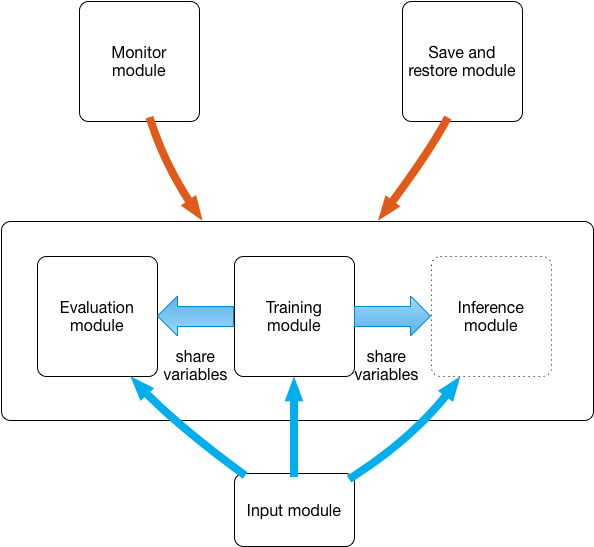
\includegraphics[width=4in]{Figures/system}
	\caption[Detail inside recurrent unit]{Illustration of recurrent network}
	\label{fig:system}
\end{figure}


\subsection{training, evaluation, inference module design}
Now let's further demonstrate the detail of the main module in Figure \ref{fig:system}. As illustrate in Figure \ref{fig:system_detail} the main module have three different sub-modules, they are training, evaluation and inference. According to different functionality, they have different components. The simplest one is the inference module. This module is only used when user already have a trained model and what to predict the secondary structures for new proteins. The only output is the prediction. The other relative simple one is the Evaluation model, this module is useful when user want to calculate the model performance on certain dataset. So beside prediction, this module also calculate the accuracy and loss. The last module is the training module, which calculate the gradient and update the correspond parameters in the model.\par

The following pseudo code is a pipeline for training a deep neural network. Generally speaking, when training a network,  it's better to evaluate the training model in real time. In this way we can save running time by early stopping the training when the model start overfitting or the improvement is really small. Comparing to the method that save a series of candidate best models. This approach also saves disk space, because at each time the system only need to keep two checkpoint files, one file records the current training process, the other records the best model which is the one with the highest validation accuracy.\par


\begin{program}
\mbox{\textbf{ Training pipeline} }
\BEGIN \\ 
\WHILE iteration \lt max\_iteration \DO 
    \CALL |training\.run\_one\_batch|()
    \IF time to validate 
        \CALL |valid_accuracy| = |validation|()
        \IF |valid_accuracy| \gt |best_accuracy|
                  \CALL |save\_model|()
                  best_accuracy = valid_accuracy\FI
    \IF \CALL |should_early|() == |True|
        break
    
\end{program}

The most straightforward way to implement the training pipeline with validation and early stopping is only build one model and switch the input dataset for training or validation. However it's not a good idea in practice. The disadvantages are the following:

\begin{enumerate}
   \item There are different input methods for data in memory and data on hard disk. In FensorFlow you can not switch between this two methods for a single model. Because the input method is part of the Graph and can not be modified once the graph finish building.
   \item If only one model is built for training and validation, the output and statistics of training and validation will be mixed together, since the monitor and output operator is also parts of the TensorFlow Graph, and can not be modified after the building phase. 
   
\end{enumerate}
So with different modules for different purposes in the graph, we can have separate input, output and monitor method for each module. When we want to train a model with validation, we can first build the training module, and then build a Evaluation module with validate dataset. And the two modules are set to share the same model parameters, to make sure the validation module are actually using learned model. When we need test result on test dataset, only a evaluation module will be build with test dataset, and the model will be initialized using saved model on hard disk.
\begin{figure}[H] 
	\centering
	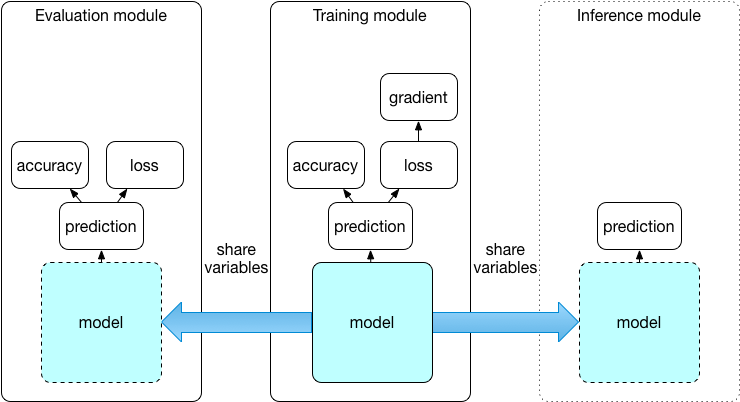
\includegraphics[width=5in]{Figures/system_detail}
	\caption[Detail inside recurrent unit]{Illustration of recurrent network}
	\label{fig:system_detail}
\end{figure}

\subsection{Implementation details}
\subsection{Input}
% introduce batch
In the network architecture discussed in Chapter \ref{CH_03}, the input is a single training example. However in practice, the input should always be a batch of multiple examples. In this case, the batch contain 64 protein sequences. And each protein sequence are normalized to 700 hundred length(protein shorter than 700 hundred pad with zeros and protein longer than 700 are cut into segments).  Figure \ref{fig:len_dist} shows the distribution of protein length, the mean value is 208, most of the proteins are shorter than 300. So in each batch, there will be more than half of the data in it are zero paddings. And these zero paddings are actual affect the performance of the network, which I will show in following sections. So in order to deal with zero paddings, besides the original input data, the length of each protein will also add to each batch. So each batch will have a shape of [64, 700, 42 + 1].

\begin{figure}[H] 
	\centering
	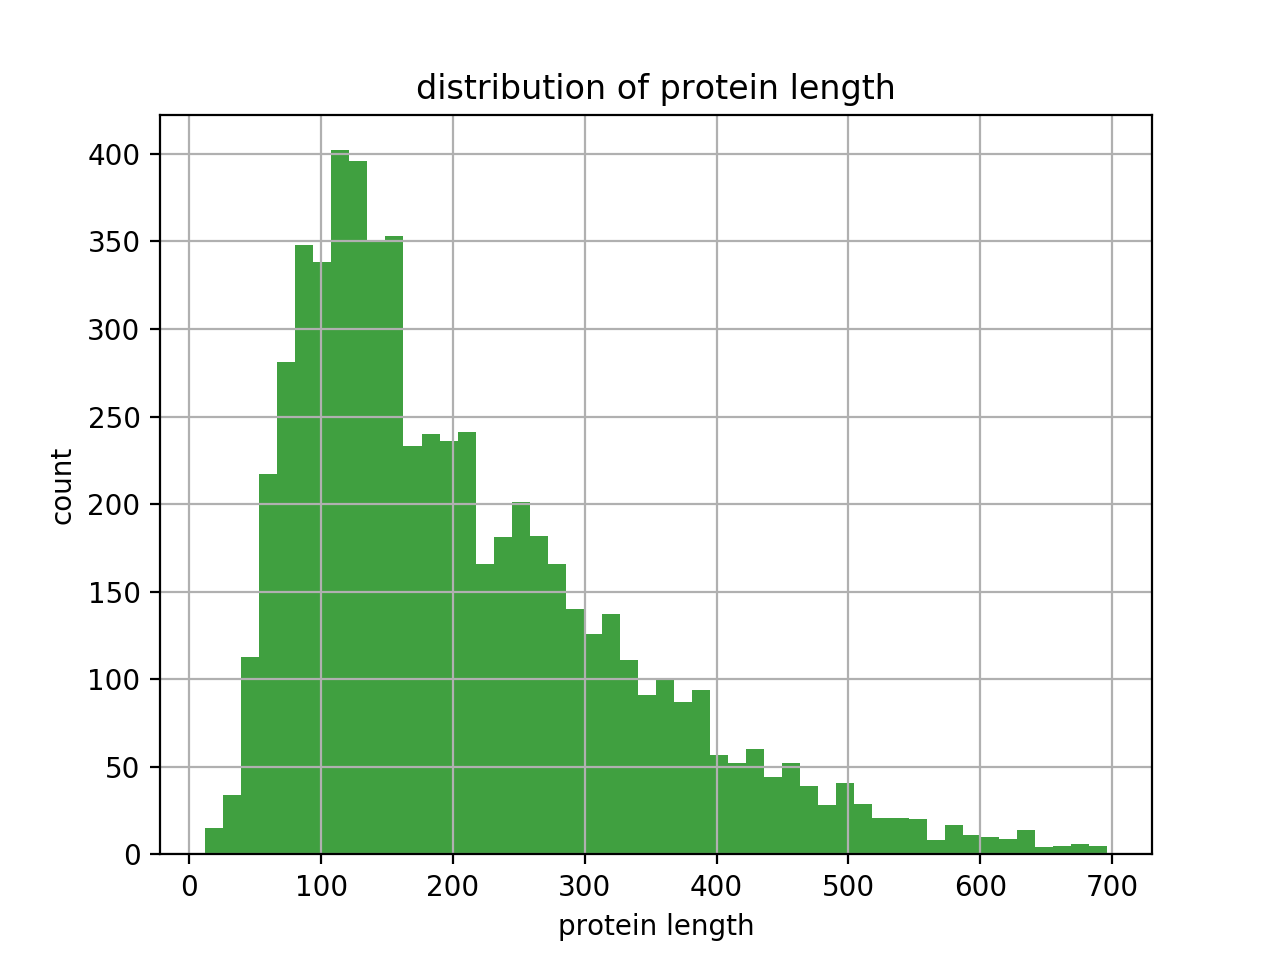
\includegraphics[width=5in]{Figures/length_distribution}
	\caption[Detail inside recurrent unit]{Illustration of recurrent network}
	\label{fig:len_dist}
\end{figure}

There are two major data input method in general. Input data from memory and input data from disk. The most popular way you will found in TensorFlow tutorials or examples are input data from memory. That is read all the data into memory and prepare each batch by your self. This method is easy to use, and user have more control of the input process. However when you can not put all the data into memory, this method is inadequate. TensorFlow also provides a build-in method for reading data from file. Users can convert all data into TensorFlows default binary format, or provide reader functions. Then TensorFlow will help you handle the data input process, as long as user provides the list of input file names. As illustrate in Figure \ref{fig:input}, a file name queue and a data queue are built as input buffer. For each step the model will read a batch from the data queue. 

In this project, training module is using the file input pipeline. However evaluation module is using the light weight memory input method, since testing and validation data are usually have small size and only need to scan through the data only once for evaluation. 

\begin{figure}[H] 
	\centering
	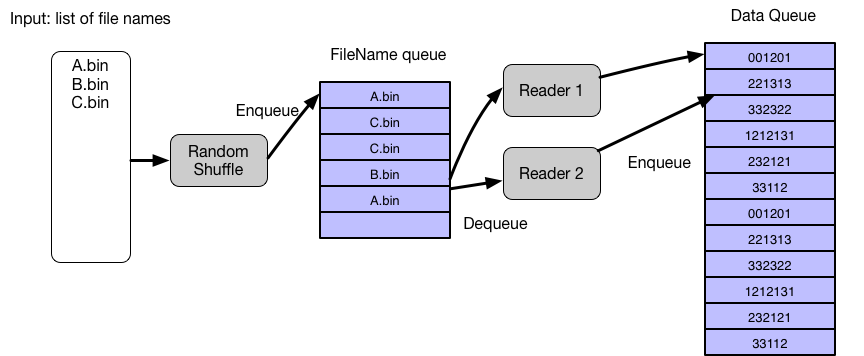
\includegraphics[width=5in]{Figures/input}
	\caption[Detail inside recurrent unit]{Illustration of recurrent network}
	\label{fig:input}
\end{figure}


\subsection{multi-scale convolution}

\subsection{recurrent layer}
When implementing the recurrent layer, there are two things should be considered. 
\begin{enumerate}
   \item Use dynamic RNN or a static RNN.
   \item When shoul RNN stop calculating for each batch.
\end{enumerate}
In TensorFlow and most other deep learning libraries, there are two common RNN versions: static RNN and dynamic RNN. Dynamic RNN is pretty much what RNN should be like, it use a loop structure to process variable lenght of sequences. The static one, however, unrolls the loop and have a fixed size of computational node to process fixed length sequences, just as what Figure \ref{fig:1} shows. \par
The benefits of using static RNN is it runs faster than a dynamic RNN, since it doesn't have to test the terminate condition for each time step. The actual speed comparison is listed in Table \ref{tb:rnn0}. What's more it is the only RNN implementation in early version of TnesorFlow. The problem of static RNN is that it makes the model too big. A big model have a lot of disadvantages. It use too much memory, both GPU and CPU memory, it consume more disk space to store the best model, and it takes more time to build the model. In this project the 700  sequence length 3 layers with 64 units model will some how use 20G memory and over 4G GPU memory. Comparing to the 4MB model file of dynamic RNN, It took 275MB to store the static model described above, which will slow down the training process every time it same the current best model. And the build time is longer than 10 minutes comparing to the several seconds of dynamic RNN's build time.\par

The reason using a dynamic RNN is that it can adapt to different input and network architectures. Such as sequence to sequence model, which needs the encoder and decoder to be able to handle variable length sequences. When dealing with real life data, a model that accepts variable length input are general easier to use. The dynamic RNN is light weight, flexible and can achieve comparable speed of a static RNN(In table \ref{tb:rnn0} the dynamic rnn is about 8\% slower than the static one).\par
\begin{table}[h] \label{tb:rnn0}
	\centering
	\begin{tabular}{lllrrr}
	\hline
	\multicolumn{3}{c}{Model} &
	\multicolumn{3}{c}{Performance}\\
	\cline{1-3}
	Multi conv & RNN  & Output layers &  Build time (s) &   \begin{tabular}{@{}c@{}}speed \\(batch/s)\end{tabular} & test accuracy(\%)\\
	\hline
	32 channels &- &conv 11  &0.69 &5.28 &65.3\\
	64 channels &- &conv 11  &0.72 &3.44 &65.7\\
	64 channels & \begin{tabular}{@{}c@{}}1 layer \\ static 32\end{tabular} &conv 11 &166.61 &0.77 &-\\
	64 channels & \begin{tabular}{@{}c@{}}1 layer \\ dynamic 32\end{tabular} &conv 11 &1.43 &0.71 &68.7\\
	64 channels & \begin{tabular}{@{}c@{}}1 layer \\ dynamic 2\end{tabular} &conv 11 &1.43 & 0.76 &67.8\\
	64 channels & \begin{tabular}{@{}c@{}}1 layer \\ dynamic 10\end{tabular} &conv 11 &1.47 & 0.758 & 68.3\\
	64 channels & \begin{tabular}{@{}c@{}}1 layer \\ dynamic 128\end{tabular} &conv 11 &1.41 &0.54 & 69.2\\
	64 channels & \begin{tabular}{@{}c@{}}2 layer \\ dynamic 128\end{tabular} &conv 11 &1.94 &0.27 &69.5\\

	\hline
	\end{tabular}
	\caption[Odd foods]{Another table which will show up in the the List of Tables as `Odd foods'; it is set to align ``here" in the text.}
\end{table}

Another important detail about RNN is when to stop the iteration. Continuing the iteration after reach the end of the sequence is inefficient, and may cause error when doing back propagation, since the network will try to learn the zero paddings that are irrelevant to the protein sequence. The problem is that proteins in each batch will have different length, so in order to stop the iteration correctly, we need to provide the length information for every protein in the batch.\par

In summary, RNN layers in this project are dynamic bidirectional RNN, and provided with sequence length information for each sequence in the batch. The unit number of the RNN cell is 128.

\subsection{output layers}
There are two 1D convolution layer are build after RNN layers. The first one use kernel shape [1] and output channel size is half of the input channel size. The second layer use kernel shape [7] and the output channel is 14.\par
\subsection{loss function}
Different from convolution networks, RNN need sevreal additional steps to calculate the correct average loss value for each batch. Because RNN always deals with variable length data, such as English sentences and ,in this project, proteins. As illustrate in Figure \ref{fig:loss} the output of the network would be a 3D array with shape [batch\_size, sequence\_length, feature\_length]. As you may notice in the figure, there are blanks at the end of each sequence, those are zero paddings. Due to the variable length input data, the blanks are always exist. And consider the distribution in Figure \ref{fig:len_dist}, over half of the data in a batch are zeros. The correct loss function for individual sequence is Equation \ref{eq:loss}. However in practice, due to the parallel feature of the system, we have to calculate the loss for all the sequence in a batch at the same time. The result of the batch loss operation is a 2D array with shape [batch, sequence]. Each element in this array is the loss of a single amino acid. After calculating the loss array, a mask array is constructed using the length vector on the left of Figure \ref{fig:loss}. Apply the mask array to the loss matrix will set the loss of the blanks to zero. Finally the average loss per amino acid will be $sum(LOSS\_ARRAY)/sum(length\_vector)$.\par

\begin{figure}[H] 
	\centering
	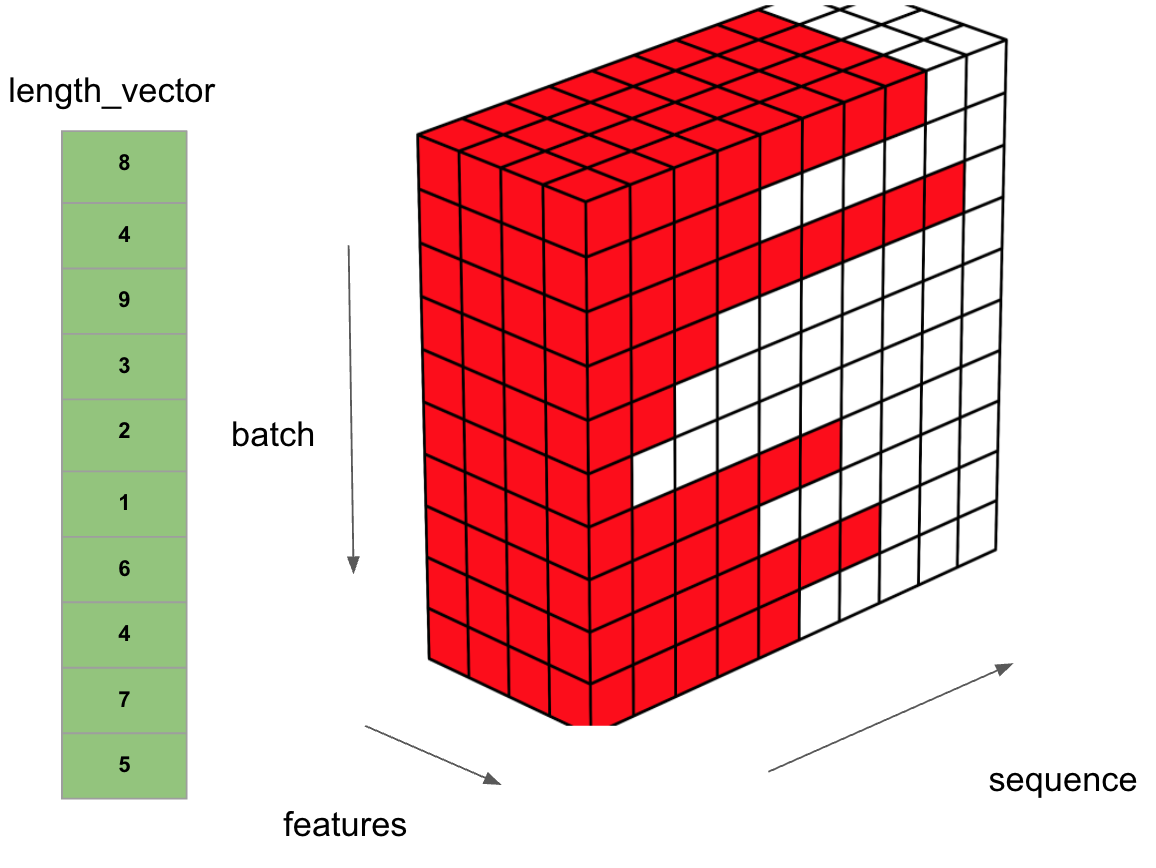
\includegraphics[width=5in]{Figures/loss}
	\caption[Detail inside recurrent unit]{Illustration of recurrent network}
	\label{fig:loss}
\end{figure}

\subsection{accuracy operator}
The evaluation of the project is 8 classes accuracy(Q8). The algorithm of calculating Q8 accuracy from predictions and labels are the following.

\begin{algorithm}[H] 
 \KwData{\\Prediction [batch\_size, seq\_len, feature\_len]\\label [batch\_size, seq\_len, feature\_len]\\length\_vector [batch\_size, 1]}
 \KwResult{Q\_8: real number}
    conf\_mat = Confusion\_Matrix(label, prediction)\;
    true\_positive = sum(diag(conf\_mat))\;
    Q\_8 = true\_positive/sum(length\_vector)\;
 \caption{Q\_8 accuracy }
\end{algorithm}

The implementation of this part is some how tricky. Because when we train the network, we want to monitor the training and validation accuracy in TensorBoard and TensorBoard only monitors the operator inside the Graph. So the whatever calculate the accuracy should be an operator inside the TensorFlow Graph. And it should not be a python function outside the Graph. So what I do here is constructing a accuracy operator using basic TensorFlow operators, and add it to the model. Then the calculation will perform inside the Graph and inside GPU. For more details see the code in Appendix.